\documentclass[a4paper,12pt]{jarticle}

% レイアウト
\setlength{\hoffset}{0cm}
\setlength{\oddsidemargin}{-3mm}
\setlength{\evensidemargin}{-3cm}
\setlength{\marginparsep}{0cm}
\setlength{\marginparwidth}{0cm}
\setlength{\textheight}{24.7cm}
\setlength{\textwidth}{17cm}
\setlength{\topmargin}{-45pt}


\renewcommand{\baselinestretch}{1.6}
\renewcommand{\floatpagefraction}{1}
\renewcommand{\topfraction}{1}
\renewcommand{\bottomfraction}{1}
\renewcommand{\textfraction}{0}
\renewcommand\thefootnote{\arabic{footnote})}

% パッケージ
\usepackage[dvipdfmx]{graphicx}
\usepackage{amsmath,amssymb,epsfig}
\usepackage{eucal}
\usepackage{bm}
\usepackage{ascmac}
\usepackage{pifont}
\usepackage{multirow}
\usepackage{enumerate}
\usepackage{cases}
\usepackage{type1cm}
\usepackage{cancel}
\usepackage{url}
\usepackage{cite}
%\usepackage{color}
\usepackage[dvipdfmx]{color}
\usepackage{caption}
\usepackage[caption=false]{subfig}
\captionsetup[figure]{labelsep=space}

% 擬似コード作成用
\usepackage[ruled,vlined]{algorithm2e}
\usepackage{setspace}
\input{../sty/jdummy.def}

% カウンタの設定
\setcounter{section}{0}
\setcounter{subsection}{0}
\setcounter{subsubsection}{0}
\setcounter{equation}{0}

% キャプションの図をFigに変更
\renewcommand{\figurename}{Fig.}
\renewcommand{\tablename}{Tab.}

% 式番号を式(章番号.番号)に
\makeatletter
\renewcommand{\theequation}{\arabic{section}.\arabic{equation}}
\@addtoreset{equation}{section}
\makeatother

% 表紙
\title{\Large{電機システム制御特論\\ レポート課題1\\ 再々提出}
% {\large No title}
}
\author{\vspace{70mm}\\
九州工業大学\ \hspace{0mm} 工学府\\
機械知能工学専攻\ \hspace{0mm} 知能制御工学コース\\
\\
所属:\ 西田研究室\\
学籍番号:\ 17344219\\
提出者氏名:\ 二宮 \hspace{0mm} 悠二\\\vspace{5mm}\\}
\date{平成29年\ 5月\ 9日}

% ドキュメントの開始
\begin{document}
% 表紙
\titlepage
\maketitle
\thispagestyle{empty}
\newpage

% 目次
\thispagestyle{empty}
\tableofcontents
\newpage

% 課題内容
\section{課題内容}
三相交流電源を持つ{\bf Fig. }\ref{circuit}の回路(三相全波ダイオード整流回路)を設計してシミュレーションを行い,
得られた出力波形から回路動作について考察する.
% その出力波形について考察する.

\begin{figure}[b]
 \begin{center}
  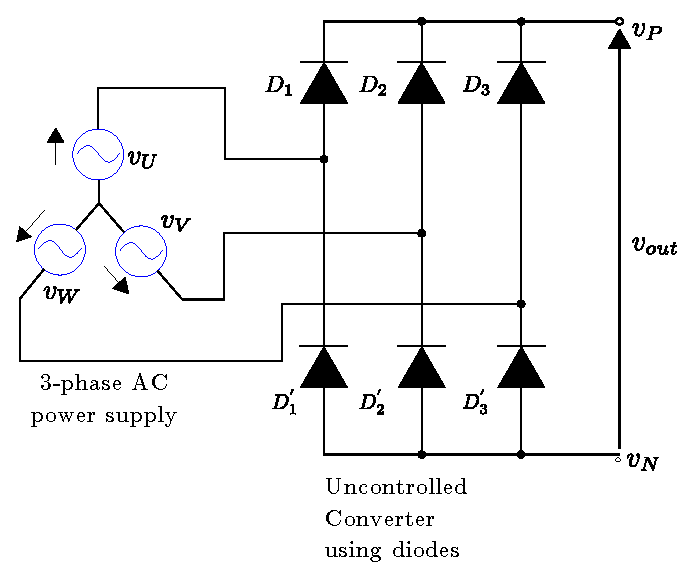
\includegraphics[scale=0.9]{../figure/circuit.eps}
  \caption{Uncontrolled converter}
  \label{circuit}
 \end{center}
\end{figure}


% 回路の説明

% \subsection{整流回路}
% 整流回路は,交流を直流に変換する電力変換回路であり,携帯電話の充電器やノートパソコンの電源アダプタ等に用いられている.本課題では,パワーデバイスとしてダイオードを用いた三相全波ダイオード整流回路について考察を行う.

\section{三相全波ダイオード整流回路} % 三相全波ダイオード整流回路へ

% 本課題にてシミュレーションを行う回路について,その仕組みを説明する.

% ・二本の配線で供給される交流電流を単相という.これに対し,三つの単相交流があり,その最大値や周波数は等しいが,交番するタイミングが互いに2$\pi/3$[rad]ずつずれているような組み合わせのものを三相交流と呼ぶ.

この回路の電源は,最大値や周波数は等しいが交錯するタイミングが互いに2$\pi/3$[rad]ずつずれている.
{\bf Fig. }\ref{circuit}において,ダイオード$D_1,D_2,D_3$はカソード側が共通に接続されており,この場合,これらのダイオードは電源電圧の正側で最も電圧が高くなる相に接続されたダイオードが導通する.したがって$v_P$にはその相の電圧が出力される.一方,ダイオード$D_4,D_5,D_6$はアノードが共通に接続されている.この場合,これらのダイオードは最も低い相のダイオードが導通するため,$v_N$にはその相の電圧が出力される.負荷電圧は上記の$v_P$から$v_N$を差し引いたものとなる.


% 三相交流とは,互いに位相角が2$\pi/3$ [rad]異なる三つの単相交流電圧,電流のことである.三つの交流電圧(あるいは電流)の振幅値が等しいときこれを対称三相交流という.とくに断りのない場合,対称三相交流を三相交流として扱う.
% 三相交流は次の理由により,発電,送配電並びに工業分野で広く利用されている.

% \begin{enumerate}
%   \item 電力を送電するとき,電線が三本で良い.したがって,電線設備費を軽減でき経済的である.
%   \item 回転磁界を容易に作ることができる.
% \end{enumerate}

% 三層電流回路のシミュレーション
\section{シミュレーション}
実際にPSIMを使用して構築およびシミュレーションを行なった回路を{\bf Fig. }\ref{circuit2}に示す.さらに,この回路から得られた電位の出力波形を{\bf Fig. }\ref{wave}に示す.なお,各素子のパラメータは{\bf Tab. }\ref{param}のように設定した.ただし,交流電源$v_U, v_V, v_W$の周波数を$f_U,f_V,f_W$,初期位相角を$\phi_U, \phi_V, \phi_W$,$v_P,v_N$間につないだ抵抗を$R$とする.また,{\bf Fig. }\ref{wave}中の補助線で区切られている1〜6の区間はそれぞれ,最高電位または最低電位の切り替わる地点で区切ったものである.これは先に述べた,どのダイオードが導通するかを示すことにあたる.これについては考察内で詳しく述べる.
\\

\begin{table}[htb]
  \begin{center}
    \caption{各素子のパラメータ}
    \begin{tabular}{c|c|c} \hline
      定数名[単位] & 記号 & 値 \\ \hline \hline
      周波数[Hz] & $f_U,f_V,f_W$ & 120 \\ \hline
                     & $\phi_U$ & $\frac{2\pi}{3}$ \\
      初期位相角[rad] & $\phi_V$ & $\frac{4\pi}{3}$ \\
                     & $\phi_W$ & $2\pi$ \\ \hline
      抵抗[$\Omega$] & $R$ & 10 \\ \hline
    \end{tabular}
    \label{param}
  \end{center}
\end{table}

\begin{figure}[tb]
 \begin{center}
  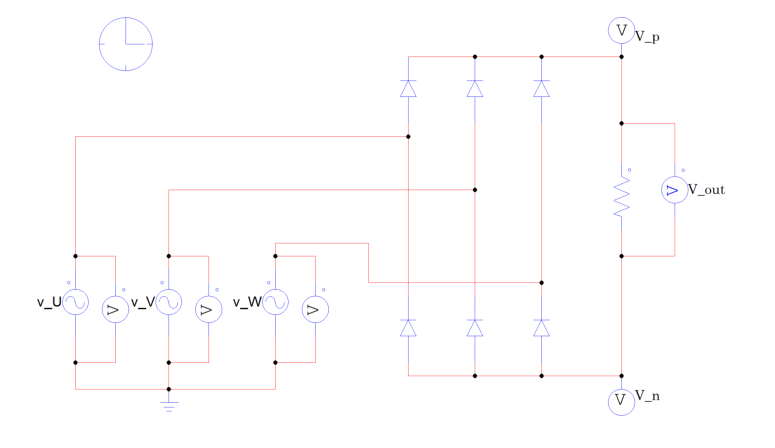
\includegraphics[scale=1.3]{../figure/circuit_rere.eps}
  \caption{PSIMにて作成した回路}
  \label{circuit2}
 \end{center}
\end{figure}

\begin{figure}[tb]
 \centering
 \vspace{0.5cm}
 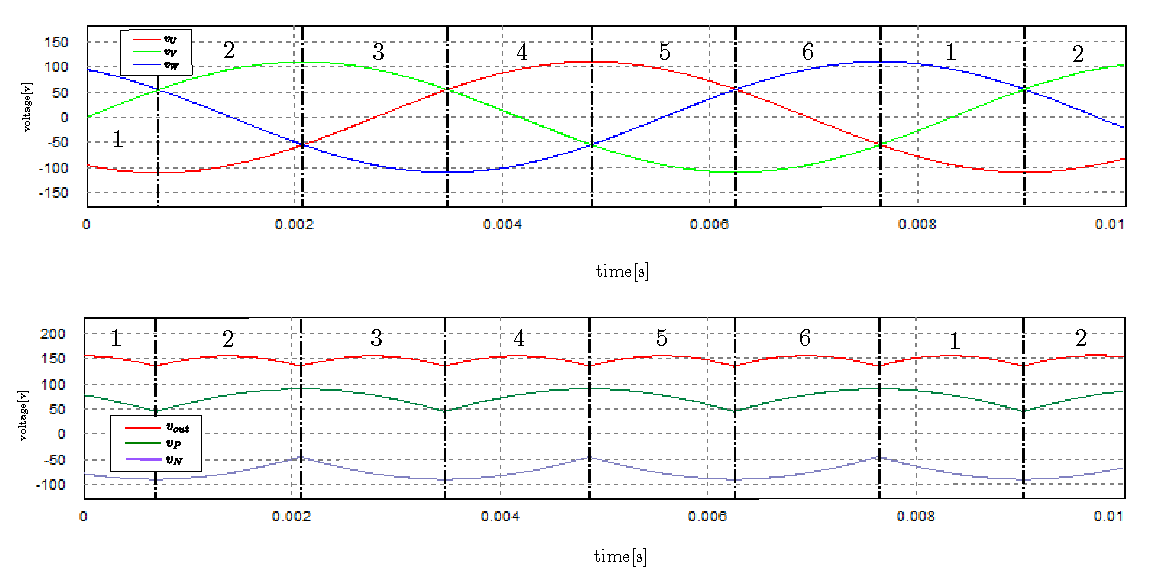
\includegraphics[scale=0.85]{../figure/waves.eps}\\
 \hspace{0.0cm}
 % 入力と出力\\
 % \\
 % \vspace{1.2cm}
 % 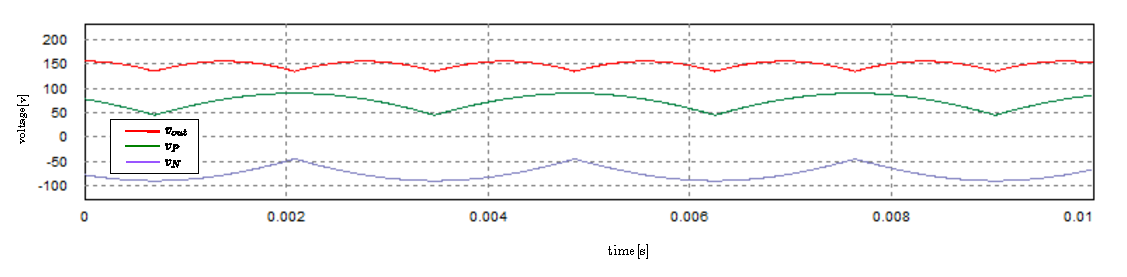
\includegraphics[scale=0.825]{../figure/output.eps}\\
 % (b) 出力の電位\\
 % \\
 \caption{シミュレーションにより得られた各電源電圧(上)と出力電位(下)の波形}
 \label{wave}
\end{figure}

\newpage

% 考察・まとめ
\section{考察}

\begin{figure}[tb]
 \centering
 \subfloat[区間1における回路動作]{\includegraphics[scale=0.5]{../figure/kukan_1.eps}}
 \hspace{1.5cm}
 \subfloat[区間2における回路動作]{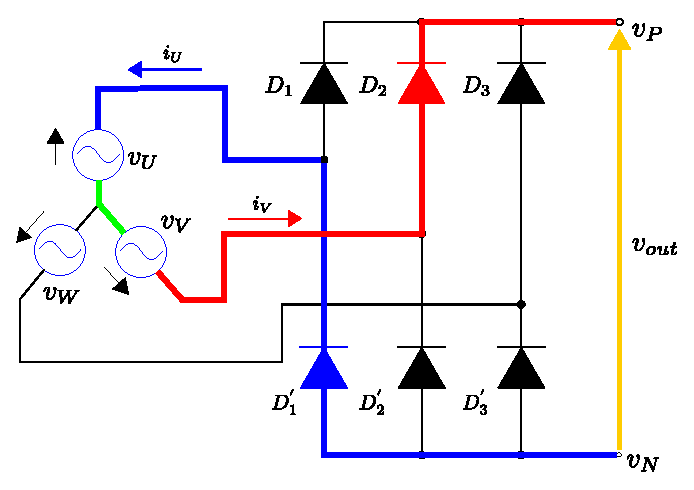
\includegraphics[scale=0.5]{../figure/kukan_2.eps}}
\\
 \vspace{0.5cm}
 \subfloat[区間3における回路動作]{\includegraphics[scale=0.5]{../figure/kukan_3.eps}}
 \hspace{1.5cm}
 \subfloat[区間4における回路動作]{\includegraphics[scale=0.5]{../figure/kukan_4.eps}}
\\
 \vspace{0.5cm}
 \subfloat[区間5における回路動作]{\includegraphics[scale=0.5]{../figure/kukan_5.eps}}
 \hspace{1.5cm}
 \subfloat[区間6における回路動作]{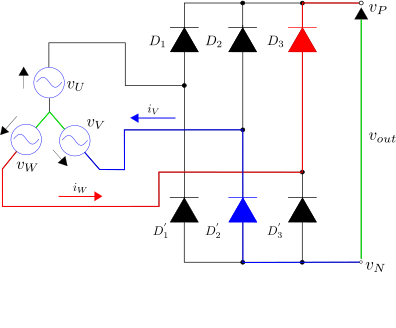
\includegraphics[scale=0.5]{../figure/kukan_6.eps}}
\\
 \caption{各区間での回路動作の様子}
 \label{circuit_kaku}
\end{figure}

% ダイオードはカソードに対するアノードの電圧を正とすると,主電流がアノードからカソードに向かって流れるようになる.
ダイオードのアノード側に正の電圧,カソード側に負の電圧を印加することを順方向バイアスをかけるといい,このとき,pn接合部において電子と正孔が結合して電荷が消滅するため,キャリアの移動が起こりやすくなりダイオードに電流が流れる.一方でその逆の場合,正孔は正の電極側,電子は負の電極側へ移動し,pn接合部で正孔と電子のやりとりが生じないため電流はほとんど流れない.したがって,
ダイオードにはアノード側からカソード側に向かってのみ電流が流れることが分かる.
本回路において,ダイオード
$D_1,D_2,D_3$からは電流が流れ出ようとするため,電圧の高い電源に繋がれたダイオードに電流が流れる.
一方,ダイオード$D_4,D_5,D_6$には電流が流れ込もうとするため,最も電圧の低い電源に繋がれたダイオードに電流が流れる.
これにより,$v_P$にはその時点で最も電圧の高くなる相の電圧が出力され,$v_N$には最も電圧の低くなる相の電圧が出力される.

以上を踏まえた上で,シミュレーションにより得られたグラフから,回路動作の様子を考察する.

{\bf Fig. }\ref{circuit_kaku}に示す六つの図は,先に示した六つの区間における回路内の動作の様子を示したものである.
% 各区間において最も電源電圧が高い相に繋がれたダイオードと,最も低い相に繋がれたダイオードに電流が流れこむため,
図中に示す赤い部分がその区間で高電位となる箇所であり,青で示した部分が低電位となる箇所である.緑は等電位を表す.これらの図から,先に述べたように回路内を電流が流れることが分かる.
また,位相が2$\pi/3$[rad]ずつずれているため,
区間1〜6の順に
% 高電位と低電位の箇所が入れ替わっていくことで,回路に交流の正の値の電流が流れ続ける.
高電位,もしくは低電位の箇所どちらか一方を残したまま,もう片方が電流の流れていない電源と切り替わることで回路に交流の正の値の電流が流れ続けることが分かる.


% したがって,$D_1,D_2,D_3$は最も電圧の高い電源に接続されたものが導通し,$D_4,D_5,D_6$は最も電圧の低い電源に接続されたものが導通する.

% 正の電極側からは断続的に正孔が供給され,同様に負の電極からは電子が補給されるため電流は流れ続ける.一方で,逆方向バイアス

% {\bf Fig. }\ref{wave}より入力と出力の関係を見ると,交流電圧のグラフのうちいずれか二つが交差している点で出力電位が下限を取り,それを堺に同じ波形が繰り返されていることが分かる.本課題では与えられたモデルと同様の回路を設計し,シミュレーションによりその出力を得た.その結果,参考とした資料\cite{1}と同様の出力波形が得られることを確認した.


% {\bf Fig. }\ref{wave}の二つのグラフを比較すると,$v_P$は三つの電源電圧のうち,電圧が最も高くなる箇所をつないだ曲線となっており,一方で$v_N$は電源電圧が最も低くなる箇所をつないだ曲線となっていることが分かる.また出力電圧$v_{out}$は$v_P$および$v_N$それぞれの波形の下限,および上限の位置を堺に,その間を一つの区間として交流波の正となる部分が繰り返されるような波形となっている.これは$v_P$と$v_N$の差を表しており,三相整流回路を形成することで,交流波の負の部分を除去し正の値のみを出力として取り出すことができるということを示している.



\section{まとめ}
本課題では与えられたモデルと同様の回路を設計し,シミュレーションによりその出力を得た.
さらにその出力波形から,回路動作の仕組みを学んだ.

% 結果,参考とした資料\cite{1}と同様の出力波形が得られることを確認するとともに,交流を直流に変換する回路の仕組みを学んだ.

\begin{thebibliography}{99}
\addcontentsline{toc}{section}{参考文献}
\bibitem{1} T.Sakamoto,”Lecture Note of Advanced Electrical Drive Control System”,pp.19-20.
\bibitem{2} 坪島 茂彦,”誘導電動機 -基礎から制御まで-”,東京電機大学出版局,pp.13-17,2006.
\bibitem{3} 横山 智紀,船渡 寛人,星 新一,吉野 輝雄,”パワーエレクトロニクス学入門”,コロナ社,pp.142-143,2009.
\bibitem{4} 高木 亮,高見 弘,鳥居 粛,枡川 重男,”基礎から分かる パワーエレクトロニクス講義ノート”,オーム社,pp.118-119,2014.
\bibitem{5} 佐藤 淳一,”パワー半導体の基本と仕組み”,秀和システム,pp.32-35,2011.
\bibitem{6} 佐藤 之彦,”パワーエレクトロニクス”,オーム社,pp.15-16,78-80,2012.
% https://www.ad.ipc.fukushima-u.ac.jp/~p142/electric/2014/13.pdf
\end{thebibliography}

\end{document}
